% Options for packages loaded elsewhere
\PassOptionsToPackage{unicode}{hyperref}
\PassOptionsToPackage{hyphens}{url}
%
\documentclass[
  9pt,
  ignorenonframetext,
]{beamer}
\usepackage{pgfpages}
% set the section number 
\setbeamertemplate{section in toc}[sections numbered]
\setbeamertemplate{subsection in toc}[subsections numbered]
\setbeamertemplate{navigation symbols}{}
% set the page
\setbeamertemplate{footline}[page number]
\setbeamertemplate{caption}[numbered]
\setbeamertemplate{caption label separator}{: }
\setbeamercolor{caption name}{fg=normal text.fg}
\beamertemplatenavigationsymbolsempty

%%
%%% Definition of colors
%%% Source: https://latexcolor.com/
\definecolor{blanchedalmond}{rgb}{1.0, 0.92, 0.8}
\definecolor{blond}{rgb}{0.98, 0.94, 0.75}
%%% End of definition of colors
%%

% Prevent slide breaks in the middle of a paragraph
\widowpenalties 1 10000
\raggedbottom
\setbeamertemplate{part page}{
  \centering
  \begin{beamercolorbox}[sep=16pt,center]{part title}
    \usebeamerfont{part title}\insertpart\par
  \end{beamercolorbox}
}
\setbeamertemplate{section page}{
  \centering
  \begin{beamercolorbox}[sep=12pt,center]{part title}
    \usebeamerfont{section title}\insertsection\par
  \end{beamercolorbox}
}
\setbeamertemplate{subsection page}{
  \centering
  \begin{beamercolorbox}[sep=8pt,center]{part title}
    \usebeamerfont{subsection title}\insertsubsection\par
  \end{beamercolorbox}
}
\AtBeginPart{
  \frame{\partpage}
}
\AtBeginSection{
  \ifbibliography
  \else
    \frame{\sectionpage}
  \fi
}
\AtBeginSubsection{
  \frame{\subsectionpage}
}
\usepackage{lmodern}
\usepackage{amssymb,amsmath}
\usepackage{ifxetex,ifluatex}
\ifnum 0\ifxetex 1\fi\ifluatex 1\fi=0 % if pdftex
  \usepackage[T1]{fontenc}
  \usepackage[utf8]{inputenc}
  \usepackage{textcomp} % provide euro and other symbols
\else % if luatex or xetex
  \usepackage{unicode-math}
  \defaultfontfeatures{Scale=MatchLowercase}
  \defaultfontfeatures[\rmfamily]{Ligatures=TeX,Scale=1}
\fi
\usetheme[]{Goettingen}
\usecolortheme{rose}
% Use upquote if available, for straight quotes in verbatim environments
\IfFileExists{upquote.sty}{\usepackage{upquote}}{}
\IfFileExists{microtype.sty}{% use microtype if available
  \usepackage[]{microtype}
  \UseMicrotypeSet[protrusion]{basicmath} % disable protrusion for tt fonts
}{}
\makeatletter
\@ifundefined{KOMAClassName}{% if non-KOMA class
  \IfFileExists{parskip.sty}{%
    \usepackage{parskip}
  }{% else
    \setlength{\parindent}{0pt}
    \setlength{\parskip}{6pt plus 2pt minus 1pt}}
}{% if KOMA class
  \KOMAoptions{parskip=half}}
  
% adjust for sidebar
  \setbeamertemplate{sidebar \beamer@sidebarside}
  {
    \beamer@tempdim=\beamer@sidebarwidth%
    \advance\beamer@tempdim by -6pt%
    \vskip4em%
    \insertverticalnavigation{\beamer@sidebarwidth}%
    \vfill
    \ifx\beamer@sidebarside\beamer@lefttext%
    \else%
      \usebeamercolor{normal text}%
      \llap{\usebeamertemplate***{navigation symbols}\hskip0.1cm}%
      \vskip2pt%
    \fi%
  }%

  \ifx\beamer@sidebarside\beamer@lefttext%
    \defbeamertemplate*{sidebar right}{sidebar theme}
    {%
      \vfill%
      \llap{\usebeamertemplate***{navigation symbols}\hskip0.1cm}%
      \vskip2pt}
  \fi

\setbeamertemplate{section in sidebar}%{sidebar theme}
{%
  \vbox{%
    \vskip1ex%
    \beamer@sidebarformat{3pt}{section in sidebar}{\insertsectionheadnumber
~\insertsectionhead}%
  }%
}
\setbeamertemplate{section in sidebar shaded}%{sidebar theme}
{%
  \vbox{%
    \vskip1ex%
    \beamer@sidebarformat{3pt}{section in sidebar shaded}{\insertsectionheadnumber
~\insertsectionhead}%
  }%
}  

\makeatother
\usepackage{xcolor}
\IfFileExists{xurl.sty}{\usepackage{xurl}}{} % add URL line breaks if available
\IfFileExists{bookmark.sty}{\usepackage{bookmark}}{\usepackage{hyperref}}
\hypersetup{
  pdftitle={BIOS6643 Longitudinal},
  pdfauthor={EJC},
  hidelinks,
  pdfcreator={LaTeX via pandoc}}
\urlstyle{same} % disable monospaced font for URLs
\newif\ifbibliography
\setlength{\emergencystretch}{3em} % prevent overfull lines
\providecommand{\tightlist}{%
  \setlength{\itemsep}{0pt}\setlength{\parskip}{0pt}}
\setcounter{secnumdepth}{-\maxdimen} % remove section numbering

%
% When using babel or polyglossia with biblatex, loading csquotes is recommended 
% to ensure that quoted texts are typeset according to the rules of your main language.
%
\usepackage{csquotes}

%
% blockquote
%
\definecolor{blockquote-border}{RGB}{221,221,221}
\definecolor{blockquote-text}{RGB}{89,89,89}
\usepackage{mdframed}
\newmdenv[rightline=false,bottomline=false,topline=false,linewidth=3pt,linecolor=blockquote-border,skipabove=\parskip]{customblockquote}
\renewenvironment{quote}{\begin{customblockquote}\list{}{\rightmargin=0em\leftmargin=0em}%
\item\relax\color{blockquote-text}\ignorespaces}{\unskip\unskip\endlist\end{customblockquote}}

%
% Source Sans Pro as the de­fault font fam­ily
% Source Code Pro for monospace text
%
% 'default' option sets the default 
% font family to Source Sans Pro, not \sfdefault.
%
\usepackage[default]{sourcesanspro}
\usepackage{sourcecodepro}

% XeLaTeX specific adjustments for straight quotes: https://tex.stackexchange.com/a/354887
% This issue is already fixed (see https://github.com/silkeh/latex-sourcecodepro/pull/5) but the 
% fix is still unreleased.
% TODO: Remove this workaround when the new version of sourcecodepro is reelased on CTAN.
\ifxetex
\makeatletter
\defaultfontfeatures[\ttfamily]
  { Numbers   = \sourcecodepro@figurestyle,
    Scale     = \SourceCodePro@scale,
    Extension = .otf }
\setmonofont
  [ UprightFont    = *-\sourcecodepro@regstyle,
    ItalicFont     = *-\sourcecodepro@regstyle It,
    BoldFont       = *-\sourcecodepro@boldstyle,
    BoldItalicFont = *-\sourcecodepro@boldstyle It ]
  {SourceCodePro}
\makeatother
\fi

\AtBeginSubsection{}
\AtBeginSection{}

\title{BIOS6643 Longitudinal}
\subtitle{L5 Contrast}
\author{EJC}
\date{}
\institute{Department of Biostatistics \& Informatics}

\begin{document}
\frame{\titlepage}

\begin{frame}
  \begin{columns}
  \column{10cm}
  \tableofcontents
  \end{columns}
\end{frame}
\hypertarget{overview}{%
\section{Overview}\label{overview}}

\begin{frame}{Topics}
\protect\hypertarget{topics}{}
\begin{itemize}
\item
  Foundational material (see other document)
\item
  Statistical models, different formulations

  \begin{itemize}
  \tightlist
  \item
    Means versus effects models
  \item
    Full rank versus less-than-full-rank models
  \end{itemize}
\item
  g-inverses and estimability
\item
  Key theorems and identities
\item
  Writing custom tests for fixed effects in the LMM
\item
  Class versus continuous predictors (e.g., time).
\end{itemize}
\end{frame}

\begin{frame}{Means versus effects models}
\protect\hypertarget{means-versus-effects-models}{}
Consider an experiment where subjects in 2 groups are observed over 3
times. Write the associated effects and means models.

\vspace{\baselineskip}
\vspace{\baselineskip}

If different subjects were observed at each \(Group \times Time\)
combination, we would have factorial data that would normally be
analyzed with 2-way ANOVA. The statistical models would look similar,
but in that case I usually write the model for \(Y_{ijk}\), where \(i\)
indexes group, \(j\) indexes time, and \(k\) replicate (right side
adjusted accordingly).
\end{frame}

\begin{frame}{Full-rank versus less-than-full-rank models:}
\protect\hypertarget{full-rank-versus-less-than-full-rank-models}{}
In 6612 you were introduced to full-rank and less-than-full-rank (LTFR)
models. The LTFR model includes a column for each level of each
categorical variable.

\textbf{Full rank approach}: Say we have a continuous variable such as
time, and 3 treatment \(Groups\ (A,\ B,\ Control)\);
\(Group \times Time\) will also be included in the model; \(X\) has 6
columns. Let \(x_1 = Time\), \(x_2=1\) for treatment \(A\), 0 otherwise;
\(x_3=1\) for treatment \(B\), 0 otherwise (\(Control\) will be the
reference group -- i.e., we have imposed a set-to-0 restriction for the
\(Control\) group). Let \(i\) denote the unique data-wide index for
subject, and \(j\) the index for \(Time\). Since times of measurement
may not be the same for subjects, I keep the \(i\) index on the time
variable as well as \(j\). The model can then be expressed as:

\[
Y_{ij} = \beta_0 + \beta_1 x_{1ij} + \beta_2 x_{2i} + 
\beta_3 x_{3i} + \beta_4 x_{1ij} \cdot x_{2i} + \beta_5 x_{1ij} \cdot x_{3i} + ε_{ij}
\]

Note that we can use like notation for all predictors, but we will have
to `manually construct' the dummy variables for treatment group. We have
a model with full rank \(X\), so don't need to worry about generalized
inverses.
\end{frame}

\begin{frame}{}
\protect\hypertarget{section}{}
\textbf{Less-than-full-rank approach}: There are 8 columns in \(X\);
let's define the treatment effects as \(\kappa_h\) for
\(Group\ 1 (A),\ 2 (B)\ and\ 3 (Control)\), and let \(\gamma_h\) denote
the \(Group \times Time\) interaction for \(h=1,\ 2\ ,\ 3\). Since there
is only one interaction term, we don't need to add another index on the
effect other than one for Group. The model is:

\[
Y_{hij} = \beta_0 + \beta_1 x_{1ij} + \kappa_h + \gamma_h x_{1ij} + \epsilon_{ij}
\]

for \(Group\ h\), \(Subject\ i\) and \(Time\ j\). The statistical model
has mixed notation, and the associated matrix has less-than-full rank
(i.e., dependency in columns).
\end{frame}

\begin{frame}{}
\protect\hypertarget{section-1}{}
In computing estimates, the issue with the LTFR models is that if we
include a column in \(\pmb X\) for each of \(c\) levels of a categorical
variable, \(\pmb X\) will not have full rank, nor will
\(\pmb {X^{\top}X}\), and hence a regular inverse cannot be used when
calculating the estimator for \(\pmb {\hat \beta}\).

Two basic approaches can be used to handle this issue.

\begin{itemize}
\item
  Force a constraint on the model up front (set-to-0 or sum-to-0), so
  that X has full rank and regular inverses can be used. I.e. create a
  full-rank model for the situation.
\item
  Introduce a new type of inverse that will handle the singularity
  issue.
\item
  In some cases these approaches are essentially the same. (E.g., SAS's
  g-inverse approach is essentially like setting the highest levels of
  factors to 0.)
\end{itemize}

\textbf{For more information, see the course notes, or refer to your
BIOS6612 material.}
\end{frame}

\begin{frame}{Estimability of \(\pmb \beta\)}
\protect\hypertarget{estimability-of-pmb-beta}{}
\begin{itemize}
\item
  For LTFR models, \(\hat \beta\) is not unique and depends on the
  g-inverse used. Theory of estimability tells us which linear
  combination of parameters are estimable in the LTFR model.
\item
  Some might find using LTFR models a little confusing, however doing so
  eliminates the need to manually create indicator variables and helps
  streamline modeling and programming code to get estimates related to
  all levels of categorical variables.
\item
  When you use the CLASS statement in PROC MIXED or PROC GLM, you are
  fitting a LTFR model.
\item
  In R, using `factor' in the lme function is like using CLASS in PROC
  MIXED, except this approach is equivalent to setting the 1st level of
  a factor as the reference, rather than the last.
\item
  To determine whether \(\pmb {L\beta}\) is estimable, see if
  \(\pmb {L=LH}\) for the \(\pmb L\) in question. If the equation holds,
  then \(\pmb {L\hat \beta}\) has a unique distribution (despite which
  g-inverse is used for \(\pmb {X^{\top}X}\)) and \(\pmb {L\hat \beta}\)
  is estimable.
\item
  When including the `e' option in the MODEL statement, SAS produces the
  form of estimable functions for generic \(\pmb L\).
\end{itemize}
\end{frame}

\begin{frame}{Linear form}
\protect\hypertarget{linear-form}{}
Consider an \(n \times 1\) random vector
\(\pmb Y \sim \mathcal N(\mu,\ \Sigma)\) where \(\Sigma\) has full rank.
For an \(m\times n\) matrix \(\pmb A\), the linear form:

\[
\pmb {AY} \sim \mathcal N (\pmb {A\mu},\ \pmb{A\Sigma A^{\top}})
\]

if \(r(\pmb A)=m\), where \(m \leq n\). Note that this is an
\(m\)-variate distribution since \(\pmb {AY}\) is an \(m \times 1\)
vector.

Example: distribution of \(\pmb {\hat \beta}\).
\end{frame}

\begin{frame}{Quadratic form}
\protect\hypertarget{quadratic-form}{}
For an \(n \times n\) matrix \(\pmb A\) and \(\pmb Y\) as before,

\[
\pmb {Y^{\top} AY } \sim \chi_\nu^2 (\lambda)
\]

where \(\lambda = \frac 1 2 \pmb {\mu^{\top} A \mu}\) is the
noncentrality parameter and \(\nu = r(\pmb A)\) are degrees of freedom
if and only if any of the following conditions hold:

\begin{enumerate}
\tightlist
\item
  \(\pmb {A \Sigma}\) is idempotent {[}i.e.,
  \(\pmb {(A \Sigma)^2 = A \Sigma}\){]},\\
\item
  \(\pmb \Sigma A\) is idempotent {[}i.e.,
  \(\pmb {(\Sigma A)^2 = \Sigma A}\){]},\\
\item
  \(\pmb \Sigma\) is a generalized inverse of \(\pmb A\).
\end{enumerate}

The distribution shown above is a non-central \(\chi^2\) distribution.
When \(\mu = 0\), we have \(\lambda = 0\), which is the central
\(\chi^2\) distribution that we're familiar with.

Example: Distribution of \(\hat {\sigma}^2\)
\end{frame}

\begin{frame}{Custom tests and estimates in the LMM}
\protect\hypertarget{custom-tests-and-estimates-in-the-lmm}{}
Researchers will (or should) have some idea about specific hypotheses
they would like to test or estimates then would like to obtain. The
inferential methods we've already learned associated with GLM's and
LMM's will help us to create custom tests and estimates. Here, we focus
on the LMM although the methods are similar in the GLM case. Below is a
quick review of the methods, followed by some examples.
\end{frame}

\begin{frame}{}
\protect\hypertarget{section-2}{}
\begin{itemize}
\item
  Likelihood ratio tests (LRT), \(F\)-tests for multiple equations

  \begin{itemize}
  \tightlist
  \item
    LRTs or \(F\)-tests can be performed for
    \(H_0: \pmb {c\beta} = \pmb h\) where \(\pmb c\) is a matrix and
    \(\pmb h\) is a vector of numbers, but usually \(\pmb 0\).

    \begin{itemize}
    \tightlist
    \item
      In SAS PROC MIXED, obtain \(F\)-tests using the CONTRAST
      statement.
    \item
      In R, equivalent LRT tests can be obtained by using the
      \textbf{anova.lme()} function that follows full and reduced lme
      fits.
    \item
      For class variables with more than 2 levels, associated main
      effect or interaction tests require \(F\)-tests.
    \end{itemize}
  \item
    Tests are more versatile than \(t\)-tests since the latter can only
    handle 1 equation at a time.
  \end{itemize}
\item
  Estimate of \(\pmb {L\beta}\) and associated Wald tests

  \begin{itemize}
  \tightlist
  \item
    \(\pmb L\) is a row vector (e.g., one row in \(\pmb c\)).
  \item
    The estimate of \(\pmb {L\beta}\) is \(\pmb {L \hat \beta}\).
  \item
    The test of \(H_0:\  \pmb{L\beta} = \pmb 0\) is carried out using
    the \(t\)-statistic \(\pmb {L\hat \beta}/se(\pmb {L\hat \beta})\).
  \item
    The estimate and test are obtained using the ESTIMATE statement in
    PROC MIXED. In R, you can obtain these by using the
    \textbf{multcomp::glht()} function in the \textbf{multcomp} package.
  \end{itemize}
\item
  The above inferential methods can be carried out on either means or
  effects models. See the text for examples of main-effect and
  interaction tests written for means models. Here, we focus on writing
  coefficients for the effects models and less on computation. More
  computational details are in the text.
\end{itemize}
\end{frame}

\begin{frame}{Writing contrasts for a two-way effects model}
\protect\hypertarget{writing-contrasts-for-a-two-way-effects-model}{}
Consider the model
\(Y_{hij} = \mu + \alpha_h + \tau_j + \gamma_{hj} + ε_{hij}\), where
\(h\) denotes \(Group\), \(i\) denotes \(Subject\), and \(j\) denotes
\(Time\). We can impose a specific covariance structure for the errors
(e.g., AR(1)) to account for repeated measures. If there are
\(2 Groups\) and \(3 Times\), then there are 12 parameters:
\(\pmb \beta^{\top}=(\mu\ \alpha_1\ \alpha_2\ \tau_1\ \tau_2\ \tau_3\ \gamma_{11}\ \gamma_{12}\ \gamma_{13}\ \gamma_{21}\ \gamma_{22}\ \gamma_{23})\)

For estimates and tests involving \(\pmb {L\beta}\), \(\pmb L\) will be
a \(1 \times 12\) vector. When we write ESTIMATE or CONTRAST statements
in SAS, the coefficients in \(\pmb L\) are broken down by factors. For
example, say we want to estimate the mean for \(Group\ 1\) at the
\(3rd\ Time\). For this,
\(\pmb L=(1\ 1\ 0\ 0\ 0\ 1\ 0\ 0\ 1\ 0\ 0\ 0)\).

In SAS we would write:

\begin{center}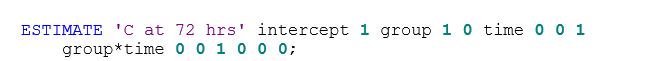
\includegraphics[width=1\linewidth]{figs_L5/f1} \end{center}
\end{frame}

\begin{frame}{}
\protect\hypertarget{section-3}{}
If certain factors do not come into play, then we do not need to include
them in the ESTIMATE or CONTRAST statement. For example, say we want to
compare means for between groups at the first time point. Then
\(\pmb L=(0\ 1\ -1\ 0\ 0\ 0\ 1\ 0\ 0\ -1\ 0\ 0)\). In SAS, the estimate
statement is:

\begin{center}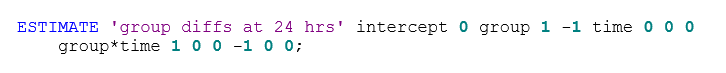
\includegraphics[width=1\linewidth]{figs_L5/f2} \end{center}

But since we have 0's for two of the factors, we can just write:

\begin{center}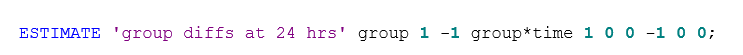
\includegraphics[width=1\linewidth]{figs_L5/f3} \end{center}
\end{frame}

\begin{frame}{}
\protect\hypertarget{section-4}{}
Note: in order to figure out how to write L above, you might find it
easier to consider each group first, and then take the difference:
\((Int\ |\ Group\ |\ Time\ |\ Group \times Time\ )\)

Control group at 24 hours:
\(\pmb L=(1\ |\ 1\  0\ |\  1\  0\  0\ |\ 1\  0\  0\  0\  0\  0)\)\\
Myostatin group at 24 hours:
\(\pmb L=(1\ |\ 0\  1\ |\  1\  0\  0\ |\ 0\  0\  0\  1\  0\  0)\)\\
Difference:
\(\pmb L=(0\ |\ 1\ -1\ |\  0\  0\  0\ |\ 1\  0\  0\ -1\  0\  0)\)

For practice: write out the null hypothesis for the main effect tests
and interaction test based on the 2-way model.
\end{frame}

\begin{frame}{Examples with real data}
\protect\hypertarget{examples-with-real-data}{}
Ramus data: The size of the ramus bone in the jaw was measured for 20
boys at 4 ages (per boy). Write the model that includes a class variable
for age and a random intercept for boy.
\end{frame}

\begin{frame}{Write polynomial contrasts for age.}
\protect\hypertarget{write-polynomial-contrasts-for-age.}{}
Some questions:

\begin{enumerate}
\item
  With 4 ages, we can go up to which degree of polynomial?
\item
  What are the coefficients for the polynomial contrasts?
\item
  What is an alternative way to write the model that will yield the same
  \(-2ln\mathcal L\) value (considering ML estimation)? Why is this?
\item
  Compare the \(F\)-test that use polynomial contrasts as rows for \(c\)
  versus the \(F\)-test that compares \(Time 1\) versus each successive
  time point. Why are they equivalent? (Full rank reparameterization
  theorem.) (It is also the same as the overall test for age.)
\end{enumerate}
\end{frame}

\begin{frame}{R code for Ramus data}
\protect\hypertarget{r-code-for-ramus-data}{}
\end{frame}

\begin{frame}{SAS code for Ramus data}
\protect\hypertarget{sas-code-for-ramus-data}{}
\begin{center}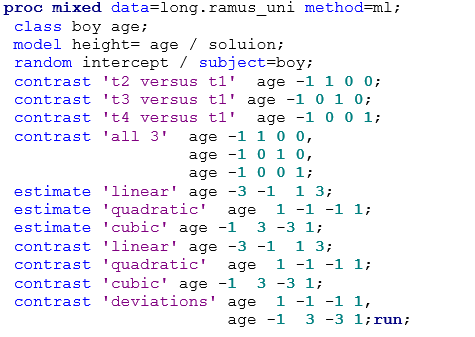
\includegraphics[width=0.5\linewidth]{figs_L5/f4} \end{center}
\end{frame}

\begin{frame}{SAS code for Ramus data}
\protect\hypertarget{sas-code-for-ramus-data-1}{}
\begin{center}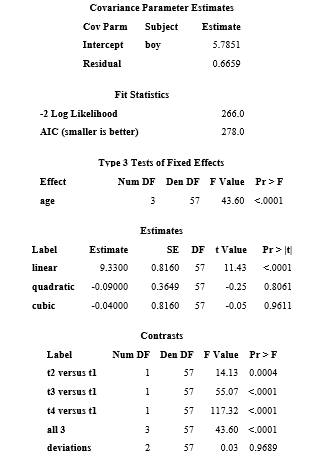
\includegraphics[width=0.5\linewidth]{figs_L5/f4.2} \end{center}
\end{frame}

\begin{frame}{Tests for interaction in the Dog data}
\protect\hypertarget{tests-for-interaction-in-the-dog-data}{}
In Sterczer, Voros, and Karsai (1996), the effect of cholagogues on
changes in gallbladder volume (GBV) in dogs was studied by
two-dimensional ultrasonography. Three different kinds of cholagogues
and tap water (administered orally) as control were used in the
experiment. Six healthy dogs were treated with each substance. GBV was
determined immediately before the administration of the test substance
and at 10-minute intervals for 120 minutes thereafter. CH=cholagogue 1
(blue), CL=cholagogue 2 (red); CO=control (green).

\begin{center}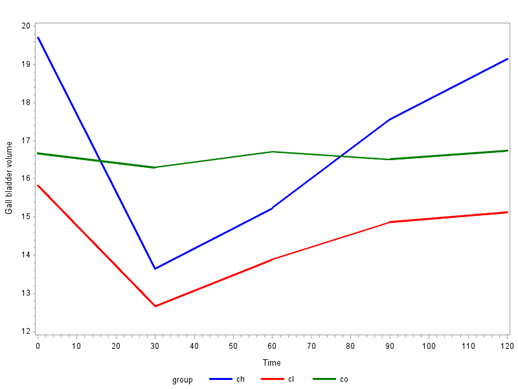
\includegraphics[width=0.5\linewidth]{figs_L5/f5} \end{center}
\end{frame}

\begin{frame}{}
\protect\hypertarget{section-5}{}
\begin{enumerate}
\tightlist
\item
  Write a model that includes group and time as class variables, plus
  group \(\times\) time interaction.
\end{enumerate}

\vspace{\baselineskip}

\begin{enumerate}
\setcounter{enumi}{1}
\tightlist
\item
  Write a test to compare is if trends over time differ between
  treatment (cholagogue) groups.
\end{enumerate}

\vspace{\baselineskip}

\begin{enumerate}
\setcounter{enumi}{2}
\tightlist
\item
  Write a test to compare changes from beginning to end among the 3
  groups.
\end{enumerate}

\vspace{\baselineskip}

\begin{enumerate}
\setcounter{enumi}{3}
\tightlist
\item
  Write a test to compare the quadratic trend of the average of
  treatment groups compared with the control. \vspace{\baselineskip}
\end{enumerate}
\end{frame}

\begin{frame}{Beta Carotene data (From Rosner, 2006.)}
\protect\hypertarget{beta-carotene-data-from-rosner-2006.}{}
A clinical trial was planned comparing the incidence of cancer in a
group taking beta-carotene in capsule form compared with a group taking
beta-carotene placebo capsules. One issue in planning such a study is
which preparation to use for the beta-carotene capsules. Four
preparations were considered: (1) Solatene (30mg capsules), (2) Roche
(60mg capsules), (3) BASF (30mg capsules), (4) BASF (60mg capsules). To
test efficacy of the four agents in raising plasma-carotene levels, a
small bioavailability study was conducted. After two consecutive-day
fasting blood samples, 23 volunteers were randomized to one of the four
preparations mentioned above, taking 1 pill every other day for 12
weeks. The primary endpoint was level of plasma carotene attained after
moderately prolonged steady ingestion. For this purpose, blood samples
were drawn at 6, 8, 10 and 12 weeks. In the plot below, the 2nd baseline
measure was used at Time 0. So in total, there are measurements at 0, 6,
8, 10 and 12 weeks.
\end{frame}

\begin{frame}{}
\protect\hypertarget{section-6}{}
\begin{center}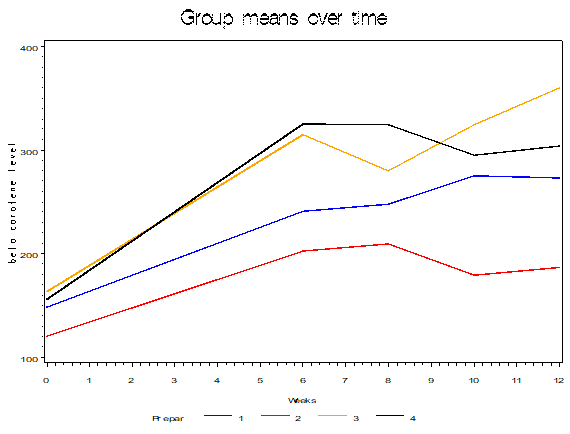
\includegraphics[width=0.5\linewidth]{figs_L5/f6} \end{center}

\begin{enumerate}
\tightlist
\item
  Look at means by time first. What are some potential models?
\end{enumerate}

\vspace{\baselineskip}

\begin{enumerate}
\setcounter{enumi}{1}
\tightlist
\item
  Write out two models, one where time is a class variable, and one
  where it is continuous.
\end{enumerate}

\vspace{\baselineskip}

\begin{enumerate}
\setcounter{enumi}{2}
\tightlist
\item
  Perform a test of interest for the model with time as a class
  variable.
\end{enumerate}

\vspace{\baselineskip}

\begin{enumerate}
\setcounter{enumi}{3}
\tightlist
\item
  Perform a test of interest for the model with time as a continuous
  variable.
\end{enumerate}

\vspace{\baselineskip}
\end{frame}

\begin{frame}{Time versus class versus continuous}
\protect\hypertarget{time-versus-class-versus-continuous}{}
\begin{itemize}
\item
  How do the estimates change if Time is treated as a continuous
  variable relative to Time as class?
\item
  If modeling Time as continuous, are higher order terms necessary?
\item
  What should you think about when deciding between Time as class versus
  Time as continuous?
\item
  In SAS PROC GLM and PROC MIXED, time can be modeled as a continuous
  variable by simply leaving the Time variable out of the CLASS
  statement (or by not using the factor argument in R).
\item
  For an indicator variable (e.g., \(0=Male\) and \(1=Female\)), do you
  need to define it as a class variable? What is the difference when you
  do or don't?
\item
  When modeling time as a class variable, the linearity assumption can
  be checked informally by inspecting graphs to see if the patterns look
  linear, or add higher order terms and see if they are significant. Can
  perform `lack of fit' test for linearity.
\end{itemize}
\end{frame}

\begin{frame}{}
\protect\hypertarget{section-7}{}
\begin{block}{Modeling time as a class versus continuous variable is an
important issue that we will discuss throughout the course.}
\protect\hypertarget{modeling-time-as-a-class-versus-continuous-variable-is-an-important-issue-that-we-will-discuss-throughout-the-course.}{}
\begin{itemize}
\tightlist
\item
  Time as a class variable\ldots{}

  \begin{itemize}
  \tightlist
  \item
    offers the most flexibility
  \item
    imposes no parametric constraints imposed across levels of time
  \item
    uses more degrees of freedom in the model (e.g., with 4 times there
    are 3 \(d.f.\), 1 \(d.f.\) if you have a simple linear term for time
    as continuous).
  \item
    recommended when there are relatively few times (say, five or less),
    for which tests for polynomial trends can still be conducted (see
    course notes for details).
  \end{itemize}
\item
  Time as continuous is recommended when\ldots{}

  \begin{itemize}
  \tightlist
  \item
    there are many times of observation, possibly unequally spaced
  \item
    there are different times of measurement for subjects
  \item
    interpolating estimates and predicted values may be of interest
  \end{itemize}
\end{itemize}
\end{block}

\begin{block}{Equivalence of model using using time as class and model
using time as continuous with \((t–1)\)th degree polynomials (if time
has \(t\) levels)}
\protect\hypertarget{equivalence-of-model-using-using-time-as-class-and-model-using-time-as-continuous-with-t1th-degree-polynomials-if-time-has-t-levels}{}
\begin{itemize}
\tightlist
\item
  Same log likelihood
\item
  Same \(F\)-test for Time
\end{itemize}
\end{block}
\end{frame}

\end{document}